%%%%%%%%%%%%%%%%%%%%%%%%%%%%%%%%%%%%%%%%%%%%%%%%%%%%%%%%%%%%%%%%%%%%%%%%%%%%%%%%
\documentclass[twocolumn]{revtex4}

\usepackage{graphicx}

\usepackage{placeins}

%%%%%%%%%%%%%%%%%%%%%%%%%%%%%%%%%%%%%%%%%%%%%%%%%%%%%%%%%%%%%%%%%%%%%%%%%%%%%%%%
% Note that comments begin with a "%" and are not turned into text in the .pdf
% document.
%%%%%%%%%%%%%%%%%%%%%%%%%%%%%%%%%%%%%%%%%%%%%%%%%%%%%%%%%%%%%%%%%%%%%%%%%%%%%%%%

%%%%%%%%%%%%%%%%%%%%%%%%%%%%%%%%%%%%%%%%%%%%%%%%%%%%%%%%%%%%%%%%%%%%%%%%%%%%%%%%
% Include some extra packages.
%%%%%%%%%%%%%%%%%%%%%%%%%%%%%%%%%%%%%%%%%%%%%%%%%%%%%%%%%%%%%%%%%%%%%%%%%%%%%%%%
%%%%%%%%%%%%%%%%%%%%%%%%%%%%%%%%%%%%%%%%%%%%%%%%%%%%%%%%%%%%%%%%%%%%%%%%%%%%%%%%

%%%%%%%%%%%%%%%%%%%%%%%%%%%%%%%%%%%%%%%%%%%%%%%%%%%%%%%%%%%%%%%%%%%%%%%%%%%%%%%%
\begin{document}

%%%%%%%%%%%%%%%%%%%%%%%%%%%%%%%%%%%%%%%%%%%%%%%%%%%%%%%%%%%%%%%%%%%%%%%%%%%%%%%%
\title{
Journal article
}

\author{Carmelo Emmanuele}
\affiliation{Siena College, Loudonville, NY}

\date{\today}

\begin{abstract}

    The motivation I had behind this final project was to see what I was capable of doing in jupyter notebook.  The programming was 	                       extremely difficult for me, but if I am ever put in a situation like this I never let it overcome me so I find the will power to complete the task.  Another motivation of mine was to see if I was able to predict the percentage of the rainfall in a month.  The first step in completing this final project was to get a better understanding of the Monte Carlo method.  The way I did this was the in-class.numpy from birthday example.  The next step to my completion of the project was to find a formula on the chance of it raining only a certain amounts of days in a month.  After I found the formula the first two problems were simple because they were basically the same question, but with two different numbers.  With the first question I defined a function and inserted a random number generator. The random number was set so if it was greater than 0 and less than equal to .2 it would return a 1.  But, if false it will return 0.  Then I made a a new def function for the number of days in a month.  In the function I called the earlier one made and added it to my list.  Lastly, took all the 1's and 0's if it equaled to 1, then it meant it only rained one day that month.  The chance of it raining only one day a month with a 20 percent chance of rain each day was .9 percent chance of it raining only one day a month.  This was the same process that I took to complete the second problem.  But, changed only two details of the code.  The first thing I changed was instead of having for loop range between 0 and .2 i changed it to 0 and .1 because now there is a 10 percent chance it will rain every day.   The second thing I changed with my code was the function of the month and instead of raining one day and one day only I changed it to be greater than or equal to 8 because it was asking the odds of it raining 8 or more days.  The second problem was asking since there is 10 percent chance of rain each day what are the odds of it raining 8 or more days.  The probability was .7 percent chance of raining 8 or more days.  The third problem was the most work done on the whole project.  In the third problem I had created 4 for loop statement to get me to my final answer.  For the first loop takes a number from 0 to number of months and in the loop are two empty lists that represent what day it rained and the other tells me yes it rained or no it didn't.  My second loop takes in the number of 0 to number of days in a month and in the loop i added to the list days that it rained with a random number generator.  With this random number generator it can tell me if it rained this day or not because it list all possible floating numbers from 0 to 1.  The third loop I have in this problem was from 3 to number of days because in the loop before i already put in the first three days, so I had to start with three.  This loop is testing to see the percentage it will rain 3 days before, two days before, and 1 day before.  And if the sequence is broken at anytime it automatically goes to 10 percent.  So if it rained 3 days before 5 percent chance, 2 days before 25 percent, 1 day before 20 percent chance of rain. My $4^{th}$ and final loop was to check how much rainfall was in that month.  It looped from 0 to number of days rained in the month.  In the loop had a random number generator and went through all days rained to see how much rain was fallen in a month.  To find the odds of it raining 10 or more centimeters was by the sum of the amount of rainfall and if it was greater than or equal to 10 it added to my first empty list total.  The final answer was 38 percent.

\end{abstract}

\maketitle
%%%%%%%%%%%%%%%%%%%%%%%%%%%%%%%%%%%%%%%%%%%%%%%%%%%%%%%%%%%%%%%%%%%%%%%%%%%%%%%%

%%%%%%%%%%%%%%%%%%%%%%%%%%%%%%%%%%%%%%%%%%%%%%%%%%%%%%%%%%%%%%%%%%%%%%%%%%%%%%%%
\section{Introduction}
%%%%%%%%%%%%%%%%%%%%%%%%%%%%%%%%%%%%%%%%%%%%%%%%%%%%%%%%%%%%%%%%%%%%%%%%%%%%%%%%

\subsection{Problem 1}
An equation used to help me solve for the first problem was $30 * .2^1 * 0.8^{29}$.  This equation means that there are 30 days in a month and I multiplied it by .2 because of 20 percent chance of rain every day raised to the 1, then multiplied that by .8 because of the chance it won't rain raised to the 29, which are how many days left in the month.  Second function used was for the month, which took in 0 to 30 days.  I had empty list called rain days I added to it to see if it would only rain one day a month.  Then, in the last two cells was where I did my actual calculations.  This was the process of getting problem number 1.

\subsection{Problem 2}
An equation used to help me solve for the first problem was $30 * .1^8 * 0.9^{22}$.  This equation means that there are 30 days in a month and I multiplied it by .1 because of 10 percent chance of rain every day raised to the 8, then multiplied that by .9 because of the chance it won't rain raised to the 22, which are how many days left in the month.  Second function used was for the month, which took in 0 to 30 days.  I had empty list called rain days I added to it to see if it would rain 8 or more days in a month.  Then, in the last two cells was where I did my actual calculations.  This was the process of getting problem number 2.
\subsection{Problem 3}

\subsubsection{3a}
For the first loop takes a number from 0 to number of months and in the loop are two empty lists that represent what day it rained and if so yes or no.  My second loop takes in the number of 0 to number of days in a month and in the loop i added to the list days that it rained with a random number generator. The third loop I have in this problem was from 3 to number of days because in the loop before i already put in the first three days, so I had to start with three.  And if the sequence is broken at anytime it automatically goes to 10 percent.  My $4^{th}$ and final loop was to check how much rainfall was in that month.  It looped from 0 to number of days rained in the month.  In the loop had a random number generator and went through all days rained to see how much rain was fallen in a month.  To find the odds of it raining 10 or more centimeters was by the sum of the amount of rainfall and if it was greater than or equal to 10 it added to my first empty list total.  


\subsubsection{3b}

\FloatBarrier
\begin{figure}[h]

\centering
	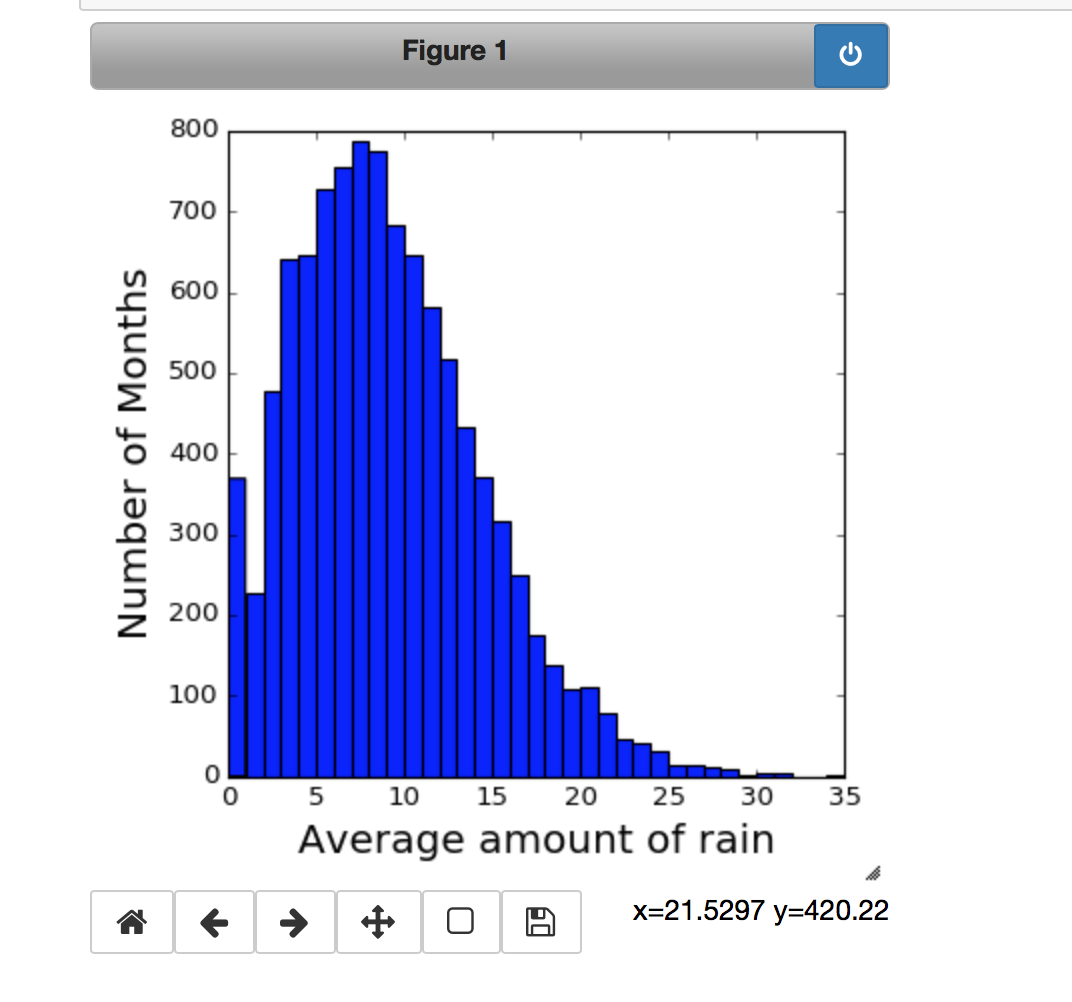
\includegraphics[width=0.5\textwidth]{Histogram}

\end{figure}	
\FloatBarrier


\subsubsection{3c}
This part of the final was the easiest because it was only two simple lines of code needed for it.  In this part of the project i had to find the average amount of rain fallen in a month.  I had to take my total list and add in the sum amount of the rain fall.  Then, I had to divide the total amount of rain by the number of the months.  Which gave me the average amount of rainfall.

%%%%%%%%%%%%%%%%%%%%%%%%%%%%%%%%%%%%%%%%%%%%%%%%%%%%%%%%%%%%%%%%%%%%%%%%%%%%%%%%
\section{Other stuff}

This final project was a rough one I had had trouble getting some of the answers.  But, after debugging the code I have finally come to some solutions that were relatively close to some answers.  I gave this my best shot and I put a lot of effort into this project.  This project was interesting to do and see the probability of the rain with one day, two days, and so-on.  Even though this was difficult to do you well prepared us for the final project.  Thanks for a fun year and now I feel confident working with python and what it has to offer me in the future.  This was a great course to take even with no programming skills what so ever!  Even though some sections of the course gave me trouble, but I worked through it till the end.  Lastly, I will still come for help throughout the time I am still in college because of the advice you gave to get through freshmen year!  Son thank you for everything!

%%%%%%%%%%%%%%%%%%%%%%%%%%%%%%%%%%%%%%%%%%%%%%%%%%%%%%%%%%%%%%%%%%%%%%%%%%%%%%%%

%%%%%%%%%%%%%%%%%%%%%%%%%%%%%%%%%%%%%%%%%%%%%%%%%%%%%%%%%%%%%%%%%%%%%%%%%%%%%%%%
\end{document}
%%%%%%%%%%%%%%%%%%%%%%%%%%%%%%%%%%%%%%%%%%%%%%%%%%%%%%%%%%%%%%%%%%%%%%%%%%%%%%%%
